\section{Test Case Generation using Deep Learning}

Our compiler test case generation approach consists of two parts: first, extending the state-of-the-art in deep learning program synthesis; the second, a general application of established differential testing methodologies for running code samples.


\subsection{CLgen}

Figure~\ref{fig:deeptune} shows the test case generation process. We extend prior work on synthetic program generation using LSTM networks~\cite{Cummins2017a}. We use a two layer LSTM network of 512 nodes each, trained for 50 epochs using an initial learning rate of XX and decaying by a factor of a half every 5 epochs.

\begin{itemize}
\item An initial seed corpus of OpenCL samples is mined from GitHub. An oracle compiler (LLVM 3.9) is used to reject samples that are not well-formed.
\item The corpus is preprocessed: a uniform code style is enforced for whitespace, braces, identifier names, etc. The prepocessed corpus is encoded using either character-level or a hybrid token/character-level encoding~\cite{Cummins2017b}.
\item LSTM networks model the vocabulary distribution over the encoded corpus.
\item The trained network is sampled to generate new programs.
\end{itemize}

%\noindent In subsequent iterations, synthesized kernels may be used to augment the training corpus.
%
%\begin{itemize}
%\item Samples are synthesized by the network and pruned using the rejection filter.
%\item The samples are mixed with kernels from the GitHub seed corpus.
%\item These combined samples are labeled (synthetic or human), and used to train a classifier for human-or-robot.
%\item The classifier is tested on unseen programs, and the accuracy is used as a fitness function for the model's parameters.
%\item A GA mutates and evolves the best performing parameters.
%\end{itemize}


\begin{figure}
  \centering
  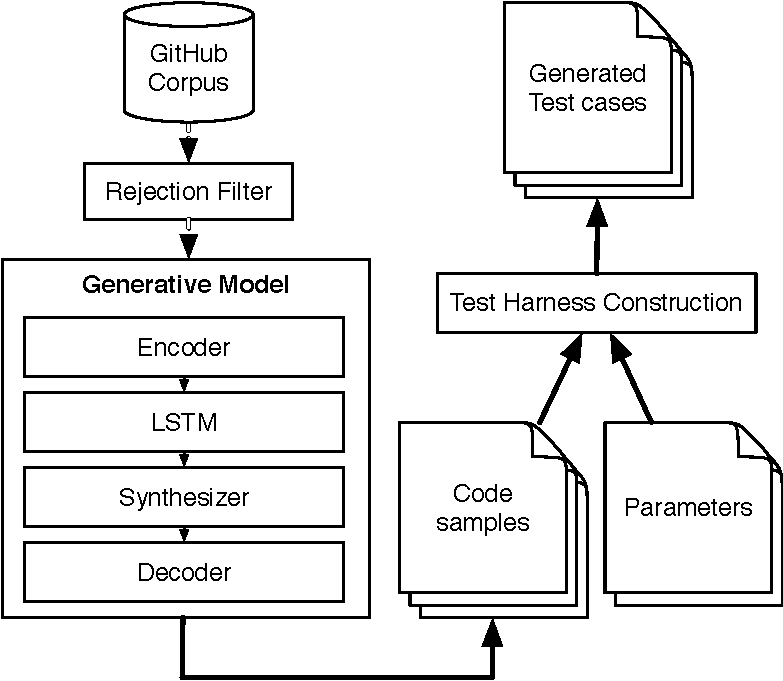
\includegraphics[width=.85\columnwidth]{img/clgen} %
  % \vspace{-2em}%
  \caption{%
    Test-case generation. An corpus of programs from GitHub is used to seed a generative model for program codes, whose outputs are parameterized to construct test cases.%
  }%
  \label{fig:deeptune}
\end{figure}

\subsection{Test Harness Construction}

At first, we used the test harness of CLSmith. However, we considered this too inflexible for our needs: CLSmith kernels accept no inputs, and compute a single result into a \texttt{unsigned long} buffer. This prototype is not a common OpenCL use case (only XX\% of GitHub kernels have this prototype). To test more a expressive range of kernels, we created \emph{cldrive}, a tool to generate test harnesses for arbitrary OpenCL kernels.

We use cldrive to generate a unique test harness for every OpenCL sample we generate; the test harness has the OpenCL kernel embedded within it. If the sample is well-formed (i.e. it can be parsed), the test harness creates a \emph{payload} of buffers and values to match the function signature; else if the sample is ill-formed we generate a compile-only stub. 

Cldrive is the only language-specific component of our software stack. We support a limited subset of data types for kernel inputs: no structs, no irregular data types (this is just an implementation detail, and can be addressed with more dev time).
